\section{Ejercicio 7 - Scheduler No Mistery}

\subsection{SchedMistery} 

Luego de experimentar arduamente con el Scheduler Mistery, hemos encontrado que implementa un esquema tipo Round Robin con múltiples colas de prioridad, utilizando un solo core.

El nivel de prioriad más alto utiliza un quantum de 1 ciclo, y además el scheduler recibe como parámetros $n$ valores que representarán el quantum de cada uno de los siguientes $n$ niveles de prioridad.

Al cargarse una tarea nueva, ésta se coloca en la cola de prioridad más alta.  Al terminar su quantum actual, cada tarea baja un nivel de prioridad y se coloca en la cola correspondiente.  Por otro lado, cuando una tarea vuelve de un bloqueo, sube un nivel de prioridad y se coloca en la cola correspondiente.

\subsection{Pruebas}

Para experimentar con el Scheduler Mistery hemos creado un nuevo tipo de tarea, a la que llamamos {\tt TaskExpMyst}. La misma recibe 4 parámetros: {\it totalcpu, lugardebloqueo, longbloqueo} y {\it cant_bloqueos}. Su funcionamiento se basa en hacer un uso de CPU de {\it totalcpu} ciclos y ejecutar {\it cant_bloqueos} bloqueos a partir del instante {\it lugardebloqueo} durando cada una {\it longbloqueo} ciclos.

Algunos de los lotes con los que experimentaron fueron:

\begin{enumerate}
\item Dos usos de CPU de 30 ciclos a partir del instante 0 y un uso de CPU de 30 ciclos a partir del instante 40.  Hemos corrido una simulación con este lote para el SchedMyst con 1 ciclo de cambio de contexto y los parámetros 4 2 6 8. Mediante este experimento hemos notado que los parámetros que recibe el scheduler son sucesivos quantums para cada tarea (salvo el primer quantum que por defecto es 1), y que cuando una tarea ingresa mientras otras están corriendo, ejecuta en forma secuencial todos los quantums hasta ``alcanzar'' el primer quantum en el que había quedado alguna de las demás tareas. En la Figura \ref{fig-1} vemos esta simulación, y podemos notar que las tareas 0 y 1 se van alternando los quantums indicados hasta el momento 44, donde ingresa la tarea 3, ejecuta los primeros 4 quantums (contando el 1) para luego seguir alternándose en la ronda las otras dos tareas.

\begin{figure}[!htb]
\begin{center}
  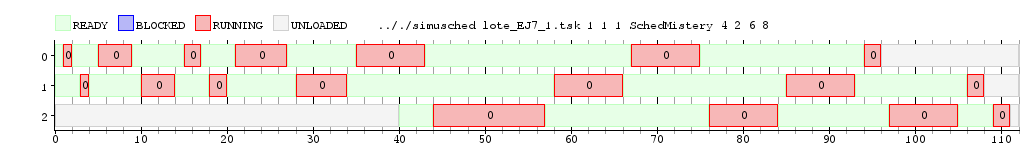
\includegraphics[scale=0.45]{imagenes/ej7-1.png}
\end{center}
\caption{Simulación lote 1 con SchedMistery, 1 ciclos de cs}\label{fig-1}
\end{figure}

\item 
\item 
\end{enumerate}

A continuación explicaremos la implementación realizada para replicar el funcionamiento del Scheduler Mistery.

\subsection{Representación}

Hemos representado las tareas con una estructura que contiene:

\begin{itemize}
\item un entero para el pid de la tarea
\item un entero para el nivel de prioridad de la tarea
\item un entero para el quantum restante de la tarea, en caso de que esté en estado {\it running}
\end{itemize}

Para implementar el scheduler, hemos utilizado los siguientes atributos:

\begin{itemize}
\item un entero que denota la cantidad de niveles de prioridad
\item un arreglo de enteros de tamaño cantidad de niveles de prioridad, donde cada entero representa el quantum correspondiente a dicho nivel
\item los datos de la tarea que está corriendo actualmente
\item una lista de tareas, correspondiente a las tareas bloqueadas
\item un arreglo de tamaño cantidad de niveles de prioridad con una cola de tareas en cada posición, representando las tareas en estado {\it ready} para cada nivel de prioridad
\end{itemize}

\subsection{Funciones}

\paragraph{Load} Se crea una nueva tarea con el pid indicado y prioridad 0, y se agrega al final de la cola de tareas correspondientes a dicha prioridad.

\paragraph{Unblock} Se recorre la lista de tareas bloqueadas hasta encontrar a la tarea con el pid indicado, se sube un nivel de prioridad (en caso de ser posible) y se agrega al final de la cola de tareas correspondientes a la nueva prioridad.

\paragraph{Tick} Se cuenta con tres casos:

\subparagraph{TICK} Primeramente se decrementa el quantum restante de la tarea actual.  Si aún tiene quantum para correr, se devuelve su pid.  En caso de que se haya terminado su quantum, se baja su nivel de prioridad (en caso de ser posible) y se agrega al final de la cola de tareas correspondientes a la nueva prioridad; luego se recorre cada cola de cada nivel de prioridad, de la prioridad más alta a la más baja, y se devuelve el pid de la primer tarea que se encuentre (que eventualmente podría ser la misma que estaba corriendo en este momento).
\subparagraph{BLOCK} Se coloca la tarea actual en la lista de tareas bloqueadas y se recorre cada cola de cada nivel de prioridad, de la prioridad más alta a la más baja, y devolviendo el pid de la primer tarea que se encuentre. Si no hay más tareas en estado {\it ready} se devuelve la constante IDLE_TASK.
\subparagraph{EXIT} Se recorre cada cola de cada nivel de prioridad, de la prioridad más alta a la más baja, y se devuelve el pid de la primer tarea que se encuentre. Si no hay más tareas en estado {\it ready} se devuelve la constante IDLE_TASK.